\chapter{Design, Methodology \& Implementation - 25\%}

\section{Design}
\subsection{Design of the Database Schema} \label{subsection:DatabaseSchema}
The design of this database schema is guided by the need to efficiently store and query data, especially as the number of function pairs scales quadratically to the number of functions in a program.

\begin{figure}[tbh!]
\centering
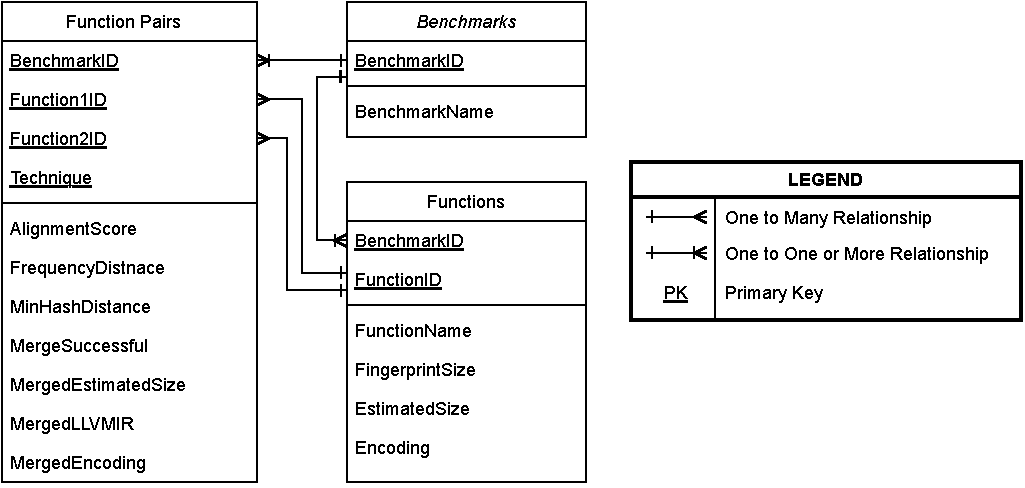
\includegraphics[scale=0.85]{Figures/DataCollectionSchema.pdf}
\caption{Schema of database used to store collected data using crows foot notation}\label{fig:DatabaseSchema}
\end{figure}

The Benchmarks table serves as the top-level reference point for all data points. This design ensures that each dataset being evaluated is logically isolated, facilitating independent analyses, comparisons, and debugging if needed.

The Functions table captures detailed information about individual functions for each given benchmark. Combining BenchmarkID and FunctionID as composite keys ensures that function identifiers are scoped locally within each benchmark, preventing cross-function ID collisions. The foreign keys ensure that each function entry is associated with a valid benchmark. 

All function metadata fields are considered optional to accommodate flexible data collection processes, depending on the user's needs. The Encoding attribute is defined with a BLOB type to store a pickled Python list representing the function's vector encoding, as discussed in sections \ref{subsection:SemanticalRepresentations} and \ref{subsection:UseOfIR2Vec}. This decision aims to reduce redundant data transformations: since the encodings are generated and used in Python (during training), storing them directly in binary format avoids unnecessary conversions to and from string representations.

Finally, the FunctionPairs table stores all function pair comparisons. The foreign keys are there to ensure that referenced benchmarks and functions exist. This table only uses a single BenchmarkID alongside two function IDs because function merging is only performed within the same program. This table also stores the distance metrics (AlignmentScore, FrequenceDistance, MinHashDistance) and Merging outcomes, where some fields are optional depending on whether the data was successfully collected. For example, we can not get the estimated size of the merged function if the merging fails.

This table stores various distance metrics (AlignmentScore, FrequencyDistance, and MinHashDistance) along with the outcomes of attempted merges. Some fields (such as MergedEstimatedSize) may be null if the merging process fails, reflecting the reasoning for allowing optional.

\subsection{Machine Learning Design}
In general, the machine learning model we are trying to develop will take in two function's embeddings as inputs and produce an alignment score as the output.

The alignment score provides a robust distance metric for function merging by capturing the structural and semantic correspondence between code sections, discussed in section \ref{METRIC:AlignmentScore}. The alignment-based approaches excel at detecting semantically equivalent code regions despite syntactic variations in the implementation. Furthermore, the score gives an early insight into the potential code size reduction achieved through merging the function pair as it measures how well two functions overlap. 

\subsection{Design of Siamese Model}
Discuss the Dot Product Siamese Model, include a diagram of the model's design
\subsection{Design of Multi-Headed Attention Model}
Discuss the Multi-Headed Attention Model, include a diagram of the model's design

\section{Methodology}
\subsection{Use of SQLite}
Prior to collecting any data, it was necessary to determine a suitable storage solution which fits the project's needs.

\paragraph{SQL vs CSV} \textbf{\textit{SQL}} databases offer significant advantages over simple file structures like CSVs primarily due to the expressive power of the SQL query language. Rather than reinventing the wheel each time a complex query is required, SQL provides a rich set of built-in functions and operators for users. This expressiveness not only simplifies the process of querying but also enhances performance, especially when working with large volumes of data, by leveraging optimised indexing and storage mechanisms. Furthermore, the relational nature of SQL databases, where data is organised into interconnected tables, enables more efficient modifications and queries across related data sets, reducing redundancy and improving maintainability.

\paragraph{SQLite vs PostgreSQL} SQLite was chosen over other SQL solutions, such as PostgreSQL primarily for its ease of use and minimal configuration requirements. Unlike PostgreSQL, which typically requires extensive set up, including robust security configurations and server management, SQLite operates as a server-less, file-based database, making it an ideal choice when sensitive data is not a concern. Additionally, its widespread adoption in the Python ecosystem offers an advantage, popular libraries like \textbf{\textit{Pandas}} and \textbf{\textit{TensorFlow}} provide support to read data from SQLite directly, further simplifying the project's implementation by enabling straightforward connections and interactions.

\subsection{Use of IR2Vec} \label{subsection:UseOfIR2Vec}
As mentioned in Section \ref{subsection:SemanticalRepresentations}, it is important to encode functions in a way that accurately captures their underlying semantics. To accomplish this, \textbf{\textit{IR2Vec}} was employed to transform the intermediate representation (IR) of each function into a 300-dimensional vector embedding. This wider dimensionality allows the encoder to capture more detail for each function and this process also produces a distinct embedding for every individual function making it a perfect fit for our needs to work at function-level granularity.

IR2Vec was selected for this project because of its ability to encapsulate the semantic meaning and flow of the IR effectively \cite{IR2Vec}. Its efficient encoding process and improved handling of out-of-vocabulary items further contribute to its appeal as an encoder. Moreover, IR2Vec is open-source and available across multiple platforms, it can be utilised as a Python library, a C++ library, or even as a stand-alone binary. This flexibility ensures seamless integration into various development environments, simplifying the overall implementation of the project.

\subsection{Data Collection and Pre-processing}
To collect the function merging data, the previous SOTA function merging implementation, F3M, was executed on a suite of benchmarks: cc1plus, chrome, libreoffice, linux, llvm, Spec2006, and Spec2007. The function merging details captured are discussed in section \ref{subsection:DatabaseSchema}.


\subsubsection{Data Imbalance}
A major challenge encountered with the dataset was the overwhelming number of function pairs with an alignment score of 0. In total, there were \textbf{\textit{2.2 billion}} function pairs collected, of which \textbf{\textit{1.67 billion}} samples had an alignment score of 0 (zero-samples), \textbf{\textit{1.7 million}} had an alignment score of 1 (one-samples) and \textbf{\textit{570 million}} has an alignment score between 0 and 1 (non-zero-non-one sample). If this imbalance is not properly addressed, the model would likely learn to predict 0 for most situations to achieve a superficially low error, but produces unhelpful predictions.

This imbalance is mitigated in two ways. First, a large portion of the zero samples is discarded so that the number of remaining zero samples equals the combined total of one samples and non-zero-non-one samples. This balancing strategy reduces the dominance of zero samples and decreases overall training time by lowering the total number of training examples. After this step, the following condition holds true:
$$Zero\ Sample = One\ Sample + Non\_Zero\_Non\_One\ Sample$$

Secondly, during model training, each remaining zero-alignment sample is assigned a weight of \textbf{\textit{0.001}}. This weighting means that every non-zero alignment sample contributes 1,000 times as much to the loss function as a zero-alignment sample, thus diminishing the influence of the overly abundant zero samples. In this way, the model is incentivised to learn accurate predictions for non-zero alignment scores.


\subsubsection{Data Split}
After collecting and processing the data, we end up with \textbf{\textit{1.1 billion}} function pairs. Then the order of data is randomised to make it diverse when encountered by the machine learning model. After which the dataset is split into three smaller datasets, the training, validation and testing datasets, each making up 70\%, 10\% and 20\% of the pre-processed dataset respectively. The training dataset is used by the model to train itself, while the validation set is used by the model to tune the hyperparameter (discussed in section \ref{subsubsection:HyperparameterTuning}). The test set is then used to test the model's performance on unseen data.

\subsubsection{Hyperparameter Tuning} \label{subsubsection:HyperparameterTuning}
Due to the sheer volume of training data available, tuning the hyperparameters using the entire training dataset would be computationally prohibitive. Therefore, a subset of 300 million training samples is used for the hyperparameter tuning stage. During this phase, a dedicated validation set is employed to evaluate each configuration of hyperparameters, ensuring that the model’s performance is robust and generalises well, not overfitting to the training data. Once the optimal hyperparameters are identified through this procedure, the model will be retrained on the full dataset comprising 1.1 billion training samples using these optimal settings.

For the hyperparameter optimisation, \textbf{\textit{Optuna}} is employed. Optuna is an efficient, automatic hyperparameter optimisation framework that utilises Bayesian optimization methods to navigate the hyperparameter space. Each evaluation of a particular set of hyperparameters is referred to as a \emph{trial}. During each trial, the model is trained on the subset of data, and its performance is measured on the validation set. The results from numerous trials guide the search process, balancing exploration of new configurations and exploitation of known good regions in the hyperparameter space, ultimately converging towards the optimal settings.


\section{Implementation}
\subsection{Artifact and Set up script}
Discuss the artifact being available and the simple set up script. Explain why IR2Vec has to be built individually by the user.

\subsection{Framework for collecting data/How to run Data Collection Scripts}
\begin{itemize}
    \item Mention how it works quite similarly for both collecting function merging details and the encodings.
    \item Talk about how it is made easy with parameterised arguments so that multiple things can run at once, and you can specify the base directory and all sub-directories are then checked for benchmarks.
    \item Talk about when getting the encodings, I had to go through the IR2Vec codebase to stop it from using the demangled name, as the F3M data collected was using the original function names.
\end{itemize}


\subsection{Pipeline for developing models}
\begin{itemize}
    \item There is one main file to train models, which handles all the loading, uses parameters to load specific models and hyperparameters for the model. 
    \item All the user has to do is to create a new model which provides the two functions, train and hyperparameter train for the two functionalities

\end{itemize}

\subsubsection{Serializing data to speed up training}
%  - Making permanent copies of Train, Validation and Testing dataset so that the steps are repeatable with the same dataeed up training
\begin{itemize}
    \item Discuss how the data was serialised to numpy values to sp
    \item Make the model run faster by serializing the data before hand and saving it using numpy.savez\_compress(). 
    \item Talk about pavlos helping and how it works.
\end{itemize}

LOADING THE SERIALISED DATA
\begin{itemize}
    \item Show the suitable chunk size
    \item Select a suitable chunk size, if not the whole system will run indefinitely.
    \item Makes use of multiprocessing in python3
    \item Each worker selects chunks of data from the database and processes the dta by deserrialising the data and then converting each chunk into a 2D ND Array, then placing it onto a queue.
    \item In the main part of the script, the 2D NDArrays are merged together and checked how many rows was processed. 
    \item Each worker checks if there is more than 20\% of the available memory before retrieving more information, if there isnt enough, it will sleep. 
    \item Now if there are the chunk size is too big, the script will not write the main chunk into files yet, and the workers will keep on waiting for the script to write the file to free up memory. This will lead to an infinite loop
\end{itemize}


\subsection{Integrating into compiler}
\begin{itemize}
    \item Mention that tensorflow model uses a C++ interface to load the model which was trained in python into the C++ compiler.
    \item  This was why the L1 Distance model was abandoned, there was a custom layer which could not be ported to the C++ without mroe engineering.
\end{itemize}

\subsubsection{Integration of IR2Vec into compiler}
\begin{itemize}
    \item Due to the difference in the LLVM/clang versions of IR2Vec and F3M codebase.
    \item So IR2Vec binary was used, encodings were stored in a text file and read from it into a lookup table when running.
    \item So newly merged function is not taken into consideration for function mering.
\end{itemize}
 

\subsubsection{Integration of TensorFlow model into the compiler}
\subsection{Use of F3M infrastructure}
\subsection{Threshold of alignment score}
\begin{itemize}
    \item Talk about how if the predicted alignment score is not the same or higher than the threshold, then the function pair was discarded, and merging was not attempted.
    \item  Multiple values were tried.
\end{itemize}




% % ==================
% \section{Data Collection}
% Prior to collecting any data, it was necessary to determine a suitable storage format to ensure robustness, scalability, and maintainability throughout the development cycle. Especially with the number of function pairs being quadratic to the number of functions in a program.

% \textbf{\textit{SQLite}} was used to store and handle all the data collected because \textbf{\textit{SQL}} is an expressive language able to facilitate complex querying compared to using CSV while still being simple enough to setup compared to other SQL systems which requires more complex setups like \textit{PostgreSQL}. Additionally, multiple python libraries provide interfaces with SQLite databases, simplifying implementation where necessary, for example \textit{Pandas} and \textit{TensorFlow} provide explicit dataloaders.\todo{CITE documentation for pandas and tensorFlow}.



% \begin{figure}[tbh!]
% \centering
% 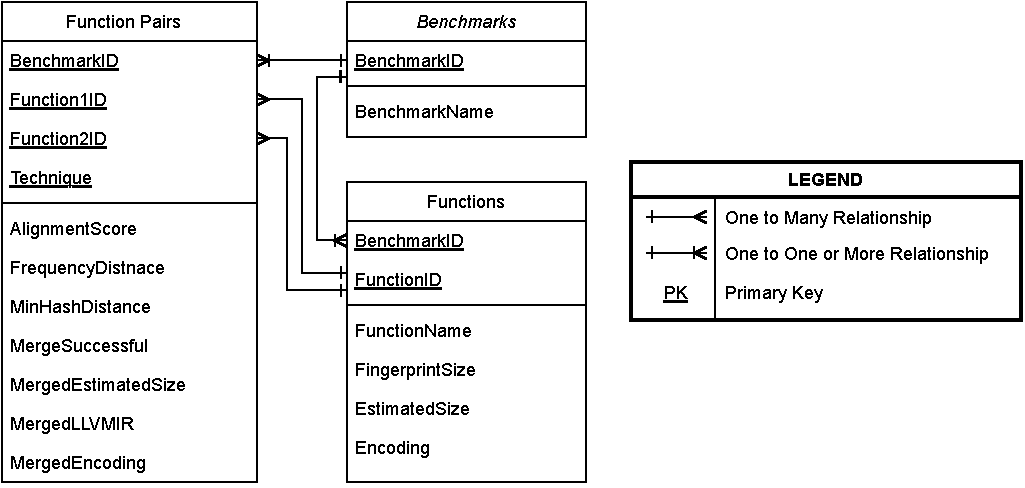
\includegraphics[scale=0.85]{Figures/DataCollectionSchema.pdf}
% \caption{Schema of database used to store collected data using crows foot notation}\label{fig:DatabaseSchema}
% \end{figure}

%  - How data is organised\\

% \subsection{Function Details}
% \begin{itemize}
%  \item Automated scripts to run the data collection, allowing for multiple data collection to run at any time, speeding it up
%  \item FunctionMerging code changes are stored in a .diff file
%  \item Explain how to use the script findBenchmarks.sh?
% \end{itemize}


% \subsection{Function Encodings}
% Talk about how IR2Vec was not working with LLVM repo, most likely because of the difference in versioning, so had to use the binary to generate function level encodings into a text file, which then had to be processed by script and placed into the database.

% The difficulty is that I had to look into the IR2Vec source code and make it use the mangled name instead of the demangled name, because the original LLVM code was using the mangled one, and it was the only way to match the encoding to the function.

% \begin{itemize}
%  \item IR2Vec is used, which uses LLVM 18.1.8
%  \item Explain how to use the script GetEncoding.py.
%  \item Choosing to store encodings as BLOB object instead of string so less time used to process data
% \end{itemize}


% \subsection{Merging Data}
%  - Explain how the script MergeDB.py works, how it merges different databases

% Had to exclude @0 and @1 function from the linux dataset, because there was no encoding?

% \section{Model}
%  - Loading data efficiently into the model
%  - Created a pipeline to run different neural network models quickly and efficiently

% \subsection{Loading Data}
%  - Efficiently Loading Data
%  - Making permanent copies of Train, Validation and Testing dataset so that the steps are repeatable with the same data
%  - Undersampling of zero alignment score samples to match the number of non-zero alignment samples

% \subsection{Dealing with Unbalanced Data}

% \subsubsection{Serializing Data}
% Make the model run faster by serializing the data before hand and saving it using numpy.savez\_compress().

% Select a suitable chunk size, if not the whole system will run indefinitely.
% Makes use of multiprocessing in python3
% Each worker selects chunks of data from the database and processes the dta by deserrialising the data and then converting each chunk into a 2D ND Array, then placing it onto a queue.

% In the main part of the script, the 2D NDArrays are merged together and checked how many rows was processed. 

% Each worker checks if there is more than 20\% of the available memory before retrieving more information, if there isnt enough, it will sleep. 

% Now if there are the chunk size is too big, the script will not write the main chunk into files yet, and the workers will keep on waiting for the script to write the file to free up memory. This will lead to an infinite loop

% \subsection{Baseline}
%  - Use Dot product on the two vectors
%  - Cosine Similarity
%  - Normalised Euclidean distance

% \subsection{L1 Distance Siamese Model}
 
% \subsection{Dot Product/Cosine Similarity Siamese Model}
% Use a Siamese model to train it to produce embeddings which will perform well when a dot product is applied to it

% Idea: Dense layer expands the 3000 dimensiona input into 512 to try to capture the more complex relationships between the two thing before compressing it down to 256, followed by 128 before checking the dot product between them.




% Does not reuse merged functions - Do not have the encodings for it


% \section{Different threshold used to not attempt all merging, waste of time}

% \section{Artifact Provided}
% With a simple set up script